\subsection{Android Application Package} \label{subsection:foundation-android-package}
Android applications are distributed and installed using the \gls{apk} file format.
They can either be obtained from an application store like Google Play, or downloaded and installed manually or by using \gls{adb}, from any other source.
The \gls{apk} format is based on the ZIP file archive format and contains the code and resources of the application.
\newline
The build process of \gls{apk} contains several steps which are visualized in figure~\ref{fig:apk}.
\newline
\begin{figure}[h]
    \centering
    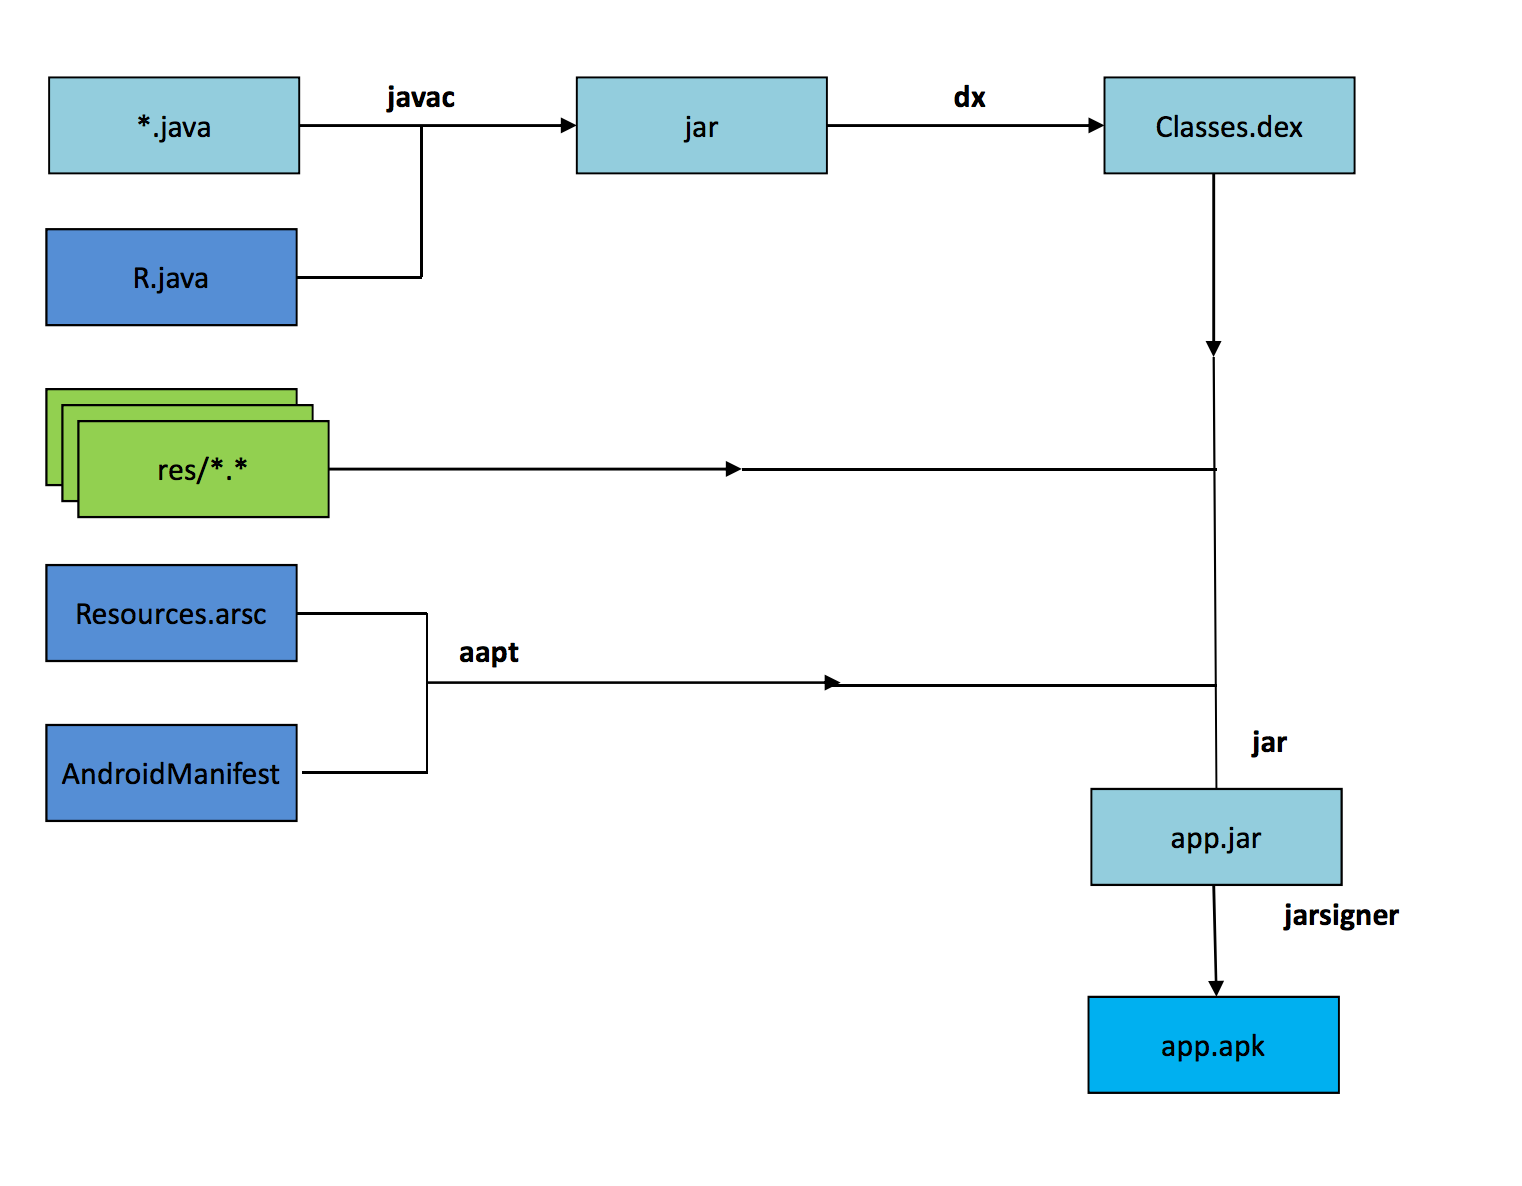
\includegraphics[width=0.8\textwidth]{data/apk.png}
    \caption{\gls{apk} build process \cite{andevconDalvikART}}
    \label{fig:apk}
\end{figure}
Since Android applications are usually written in Java, there are similarities to the Java program build process.
Upon compilation, the source code is transformed into \gls{classg} files by the Java Compiler javac.
Each Java class is stored as bytecode in the corresponding \gls{classg} file.
Java bytecode can recompiled to become readable.
To prevent that, obfuscation can be applied as described in section~\ref{subsection:counter-improve-obfuscation}.
When all Java classes are compiled to \gls{classg} files, they are packed into a \gls{jar} file.
\newline
Android uses a \gls{vm} different from Java.
It requires the Java bytecode to be converted to a different format - the Dalvik bytecode.
The Android \gls{sdk} provides \textit{dx}, the tool used to convert \gls{classg} files to a single \textit{classes.dex} file.
The \gls{vm} and the \gls{dex} file format will be described in the following.
\newline
The \gls{apk} itself consists of three parts.
\begin{itemize}
\item \textit{classes.dex}, a file containing the bytecode
\item resource files (\textit{res/*.*}), a directory containing static content like images, the strings.xml and the layout.xml files
\item resources.arsc and AndroidManifest.xml, containing compiled resources respectively essential information as required permissions
\end{itemize}
The \textit{apkBuilder} combines these files into one archive file.
\newline
Before releasing the application, it has to be signed and zipaligned.
The \textit{jarsigner} is used to sign the application.

It is done similar to the Java code signing \cite{codeSigning} by adding a manifest, a signed manifest and the certificate.
It is signed by the developer's private key and thus ensures the integrity and authenticity of the \gls{apk}.
Tampering can be detected and updates for applications with the same name and certificate can be installed.
Afterwards \textit{zipalign} is used to mark uncompressed data. \cite{androidPublishSign}  \cite{androidSigning} \cite{andevconDalvikART}
\newline
\newline
The structure of a final \gls{apk} file has the following content as minimum seen in figure~\ref{fig:apkfolder}.
\begin{figure}[h]
    \centering
    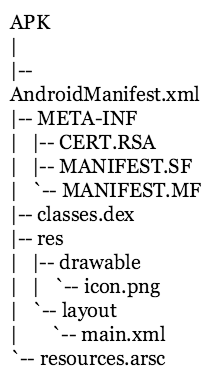
\includegraphics[width=0.5\textwidth]{data/apkfolder.png}
    \caption{\gls{apk} folder structure}
    \label{fig:apkfolder}
\end{figure}
The \textit{AndroidManfiest.xml} and the \textit{classes.dex} have already been covered.
\newline
The \textit{META-INF} folder is inherited from Java. It is used to store to store the signing information, e.g. the manifest and certificate \cite{codeSigning} \cite{metaJava}.
\newline
While the static resources, like drawables and layouts, are in the res folder, the resources.arsc contains the compiled resources.
\newline
Native libraries are written in C or C++ in order to boost performance and allow low level interaction between applications and the kernel by using the \gls{jni}.
They are stored as \textit{*.so} files in the libs folder sorted by their specific architecture, like armeabi-v7a for ARM or x86 for Intel processors.
\cite{kovachevaMaster} \cite{ehringerDalvik}
